\def\CTeXPreproc{Created by ctex v0.2.12, don't edit!}\documentclass[twocolumn,showpacs,twoside,10pt,superscriptaddress,prl]{revtex4}
%\documentclass[showpacs,twoside,10pt,superscriptaddress,prl]{revtex4}

\usepackage{graphicx}
\usepackage{epsfig}
\usepackage{epsf}
\usepackage{amssymb}
%\usepackage{epstopdf}
\usepackage{amsmath}
\usepackage{amsthm}
\usepackage{multirow}
%\usepackage[colorlinks=true,dvipdfm]{hyperref}

\newcommand{\bra}[1]{\langle #1|}
\newcommand{\ket}[1]{|#1\rangle}
\usepackage[usenames]{color}
\definecolor{Red}{rgb}{1,0,0}
\definecolor{Blue}{rgb}{0,0,1}

%opening
\pacs{03.67.Lx,07.57.Pt,42.50.Dv,76.60.-k}

\begin{document}

\title{Simulate the $H_2$ Molecule on an NMR Quantum Computer}
\author{Jiangfeng Du$^{\ast}$,Nanyang Xu, Xinhua Peng, Pengfei Wang, Sanfeng Wu, Dawei Lu \\
\normalsize{Hefei National Laboratory for Physical Sciences at
Microscale and Department of Modern
Physics,University of Science and Technology of China, Hefei, Anhui 230026, People's Republic of China}\\
\normalsize{$^\ast$To whom correspondence should be addressed;
E-mail:  djf@ustc.edu.cn}}



\begin{abstract}
The difficulty to calculate molecular energies in quantum chemistry
with classical algorithms grows exponentially with the size of
molecule. But quantum computers dramatically reduce the complexity
of this problem. We made a demonstration of simulating $H_2$
molecule in an NMR quantum computer to calculate the energy of its
ground state. We use the iterative method to get more precise bits
of the value and for each iteration we utilized the NMR
interferometry to get the energy information. Finally we get 17
precise bits of the energy value. Besides, we also show the
bottleneck of such quantum algorithms where the precision upper
bound limited by the imperfection of the operators in experiment.

\end{abstract}
\maketitle

Quantum computer have been shown in principle more powerful than
classical computers in many problems. The most famous example is the
factoring problem, which has a polynomial complexity in the Shor's
quantum factoring algorithm\cite{shor_algorithm} while no efficient
classical method is available till now\cite{knuth}. Another type of
classically hard problem is the simulation of real quantum
systems\cite{lloyld_univsim}. On classical computers, simulation of
$Sch\ddot{o}dinger$ equation of a quantum system need an
exponentially growing resource with the size of the system. In 1982,
Feynman proposed that quantum systems may be well simulated by a
quantum computer\cite{feynman}. Then S. Lloyd show that an universal
quantum computer could simulate other quantum systems efficiently.
Sequently a few demonstrated examples were shown to simulated the
small quantum systems such as oscillators\cite{oscillator},
Many-Body Fermi Systems\cite{manybody}, Heisenberg spin
chain\cite{peng2005} and \emph{etc.}.


The main task in computational quantum chemistry is to calculate the
molecular properties. The difficulty for calculation of the
molecular energies with classical algorithms scales exponentially
with the molecular size\cite{molenergy}. Recently in 2005,
Aspuru-Guzik and Dutoi \emph{et al.} (AD)\cite{molenergy} proposed a
new algorithm to simulate the molecules in quantum computers, which
could calculate the energy of the molecule with polynomial
resources. The algorithm transferred the energy information to the
phase of the quantum states and adopted a quantum phase estimate
algorithm to measure the relative phase shift of the state, and the
process is iterated many times to get more precision of bit from the
molecular energy. They use the $H_2O$ and $LiH$ molecules as
examples to show the usefulness of their algorithm, which need at
least 12 and 15 qubits in realizations. However, this requirement
excess the ability of today's quantum computation technology, so no
such experiment have been done till now.

In this letter, we firstly simulate the $H_2$ molecule in experiment
and calculate the ground energy to a precision of 17 bits. For this
work, we use the interferometry for the evaluation of the phase
shift and adopt similar iterative scheme as in the AD's proposal. we
also find that the precision of the result got from this algorithm
limited by the imperfection of operators in experiments.



As shown in Fig.\ref{circuit_exp}a, the general routines to
calculate the molecular ground energy in AD's proposal have four
steps: 1) map the molecular wave function to the qubits' space; 2)
apply the molecular Hamiltonian on the qubits which are prepared in
its ground state to generate only phase shift on the qubits; 3)
measure the phase shift and extract the energy information. 4)
iterate the procedure more time with compensating the value get from
the above loops to get more precise bit from the energy. For the
scheme we implemented in the experiment, We will introduce the later
three steps first and leave the chemistry issues behind.

In the second step, the quantum simulator's work qubit is prepared
by Adiabatic State Preparation (ASP) to $|\Psi\rangle$, the ground
state of the molecular Hamiltonian $H$. An unitary operator
$U=e^{-iH\tau}$ is applied to the state $|\Psi\rangle$, with only
generating a phase shift to the ancillary qubit by the controlled
operation. Here
$U|\Psi\rangle=e^{-iH\tau}|\Psi\rangle=e^{i2\pi\phi}|\Psi\rangle$
where $E=-2\pi\phi/\tau$ is the energy of $H$'s ground state. Note
that the energy $E$ is negative so we make the phase $\phi$ to be
positive and $\tau$ is chosen properly to make the phase $\phi$
ranges from 0 to 1.


In the measurement step, originally a four-bit inverse Quantum
Fourier Transform (QFT) is adopted as the Relative Phase Measurement
to evaluate the phase shift to get the energy value. This apparatus
need four qubits as ancilla to get on precise bit with successful
possibility of $15/16$\cite{qcqi}. However, it is hard to handle so
many extra qubits in today's technology. At the same time, in the
NMR platform there's a mature technology NMR interferometer, named
from the similar apparatus originally used in optics, which could
easily measure the relative phase shift of the quantum
states\cite{du_geophase,peng_comple}. The principles of NMR
interferometer is shown in Fig.\ref{circuit_exp}b. Very similarly
with the optical area, the NMR interferometry measures the phase
shift by modulating the spectrum patterns and the phase shift could
be evaluated with an error bound of $\pm5^\circ$ in our experiment,
much more precise than the performance of the original four-bit
inverse QFT apparatus. Thus we utilize the interferometry to measure
the phase shift in our experiment.


For a useful application in the quantum chemistry, the precision of
the energy should be extendable, so the above process should be
iterated to get more precise bits from the real value. We made a
little modification to the original AD's proposal to improve its
reliability. In our experiment for the $k$th iteration we perform
the measurement, we get the phase shift $\phi_k$ with an error bound
of $\pm\phi_{errbd}$. Then we perform the $(k+1)$th iteration by
choosing another operator $U_{k+1}=[e^{-i2\pi\phi^{'}_0}U_k]^{2^n}$,
where $n$ is the number of extra bits we want to attain in the
$(k+1)$th iteration. Of course $n$ is limited by the error bound in
the experiment. Here $\phi^{'}_k=max\{\phi_k-\phi_{errbd},0\}$. This
is because we have to make sure that $\phi^{'}_k$ is less than the
theoretical value of $\phi$ which is generated by the operator $U_k$
in each iteration and if $\phi_k$ is less than error bound then no
phase is necessary to be eliminated. Initial the iteration begins
with $U_0=U$, and by iterate the procedures, the energy value could
be accurate with a large number of bits.

However, the precision of the measurement could not be arbitrarily
high, because the imperfection of the experimental operations. To
get the $k$th bit of the energy, we have to perform the operator $U$
 with $2^k$ times, so the error of operator $U$ scales exponentially
 with the bits of precision. So in experiments, the precision of the
 energy we got relies on the precision we could perform the
 operators.



For the chemistry issues, because of the limitation in quantum
computation technologies, to calculate a large molecule's energy in
not possible for the time being. So we choose to calculate the
ground energy of $H_2$ molecule for our demonstration. The
Hamiltonian of $H_2$ molecular is shown as follows,
$$
    H=\Sigma_i(T_i+\Sigma_j{V_{ij}})+\Sigma_{i>j}{O_{ij}}
$$
where $T_i$ is the kinetic energy of electron i, and $V_{ij}$ is the
coulomb potential energy between the $i$th electron and the $j$th
nucleus, while $O_{ij}$ is the coulomb potential energy between
electrons $i$ and $j$. Here we choose the simplest situation: $H_2$
in the minimal STO-3G basis. In this two-nucleus and two-electron
molecule, each atom has a $1s$ Guassian-type function, and the two
functions compose one abonding orbital with gerade symmetry and one
antibonding orbital with ungerade symmetry. So there are 4 spin
orbital and these 4 spin orbital can form 6 configurations.
Considering the singlet symmetry and the spatial symmetry of $H_2$
exact ground state, only two configurations are acting in fact in
the calculation: the ground state configuration $|\Psi_0\rangle$ and
the double excitation configuration
$|\Psi_{1\bar{1}}^{2\bar{2}}\rangle$. Thus, the Hamiltonian matrix
is(in atom units, the nucleus distance is 1.4\emph{a.u.}, only the
electron's energy) :\cite{quantchemistry}


\begin{eqnarray}
        H&=&
        \begin{pmatrix}
            \langle\Psi_0|H|\Psi_0\rangle & \langle\Psi_{1\bar{1}}^{2\bar{2}}|H||\Psi_{1\bar{1}}^{2\bar{2}}\rangle\\
            \langle\Psi_{1\bar{1}}^{2\bar{2}}|H|\Psi_0\rangle & \langle\Psi_{1\bar{1}}^{2\bar{2}}|H|\Psi_{1\bar{1}}^{2\bar{2}}\rangle
            \end{pmatrix}\nonumber\\
        &=& \begin{pmatrix}
            -1.8310 & 0.1813\\
            0.1813 & -0.2537
            \end{pmatrix}
\end{eqnarray}
whose theoretical eigenvalue is -1.8516 \emph{a.u.}.

%=================================experiment part=======================================================
\begin{figure}[htb]
\begin{center}
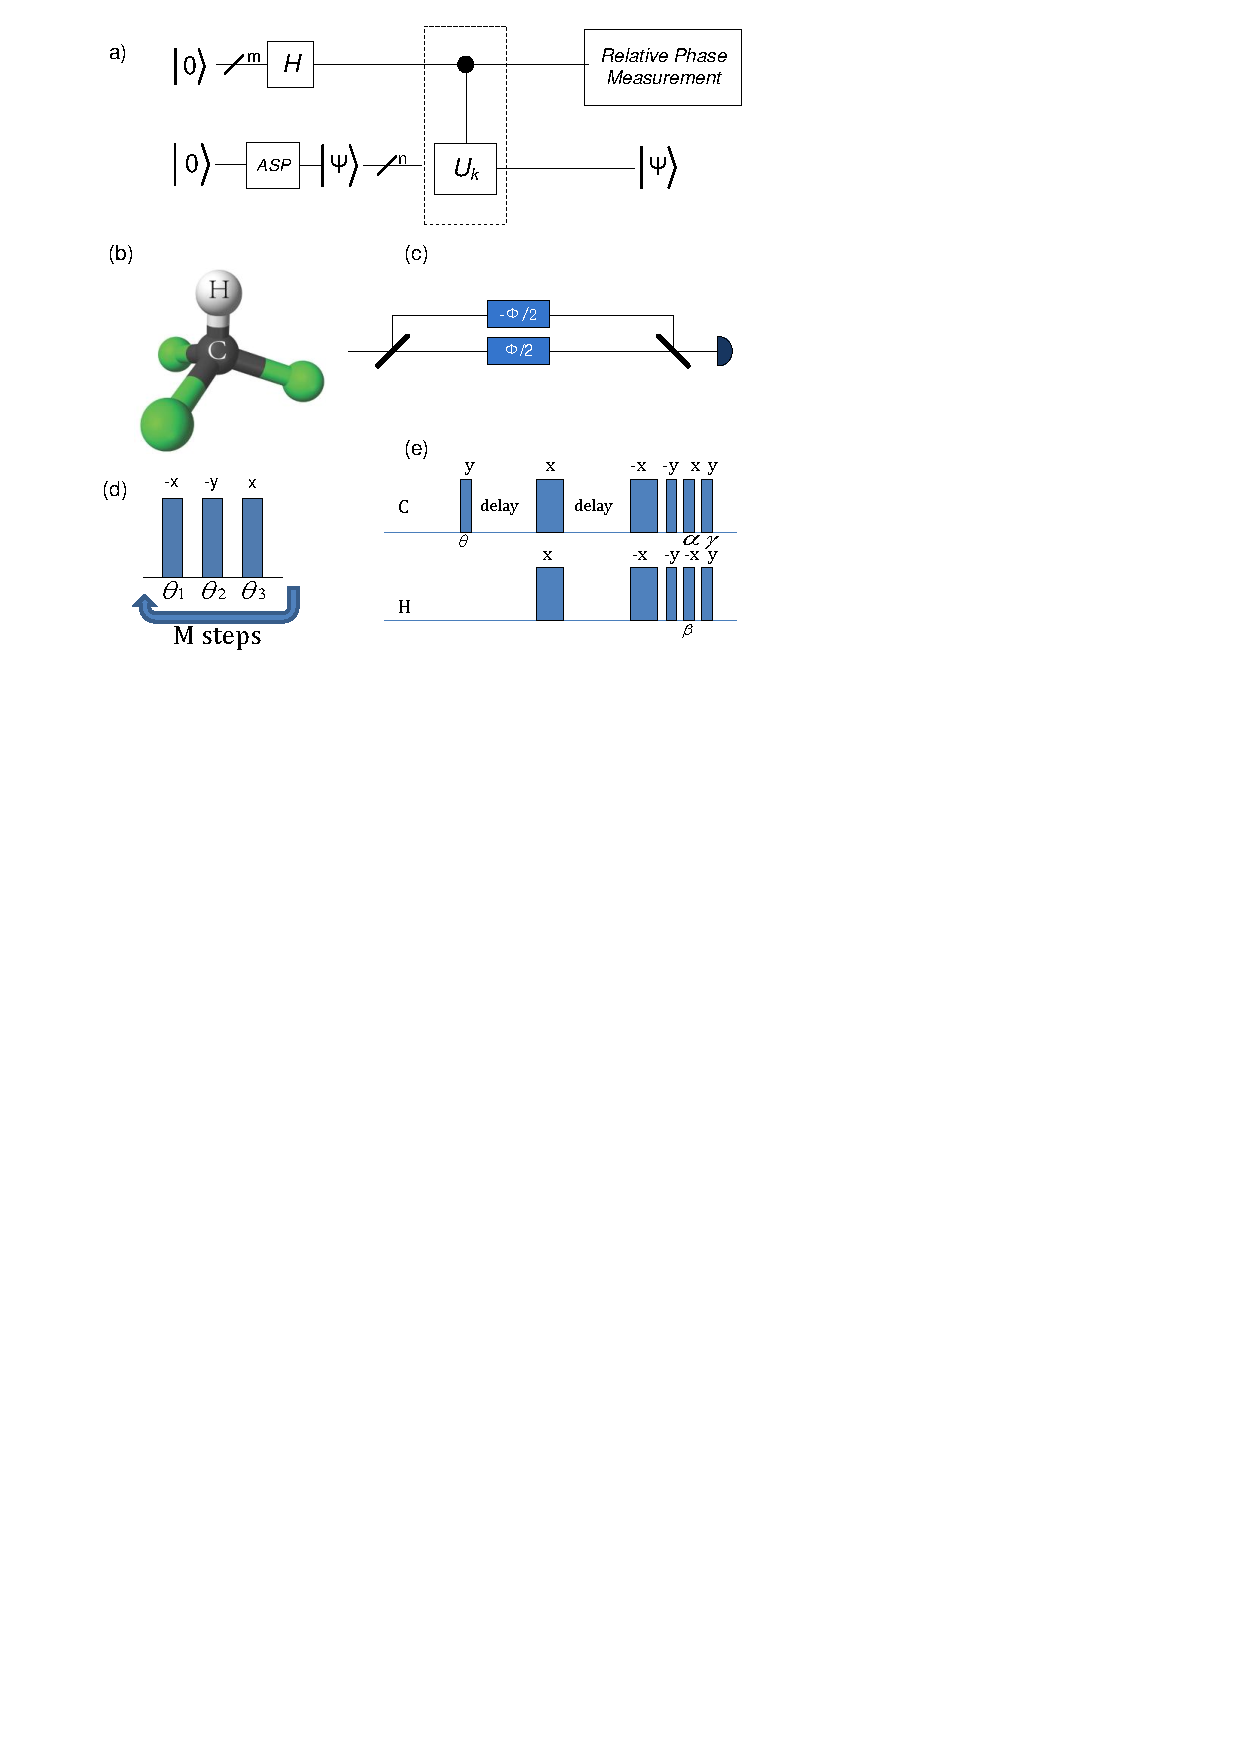
\includegraphics[width= 0.99\columnwidth]{circuit_exp}
\end{center}
\caption{(a) general schematic circuit for calculating molecular
energies. (b)The sample used in experiment $CHCl_{3}$. $^{13}C$
nucleus is used for the work qubit while $^{1}H$ is for ancillary
qubit. (c) Principle of NMR interferometry, which is used for the
Relative Phase Measurement section in our experiment. (d) The pulse
sequence to implement the Adiabatic State Preparation (ASP) process.
After ASP, the $^{13}C$ nucleus is prepared in the state
$|\Psi\rangle$--the ground state of the Molecular Hamiltonian
$H$.(e) The pulse sequence to implement the controlled-$U_k$
operation.}\label{circuit_exp}
\end{figure}

Now, we start to realize this simulation in a two-qubit NMR quantum
computer. The two qubits are represented by $^{13}C$ and $^{1}H$
nuclear spins in the chloroform ($CHCl_{3}$),respectively. The
molecular structure is shown in Fig.\ref{circuit_exp}b, where the
two qubits are marked out. The natural Hamiltonian of this two-qubit
system is:
\begin{eqnarray}\label{HamCHF}
\mathcal{H}_{\mathit{NMR}}=\frac{\omega_{H}}{2}\sigma_{z}^H+\frac{\omega_{C}}{2}\sigma_{z}^{C}+\frac{\pi
J_{CH}}{2}\sigma_{z}^{H}\sigma_{z}^{C}
\end{eqnarray}
where $\omega_{H}/2\pi$ and $\omega_{C}2\pi$ are the Larmor
frequencies and $J_{CH}$ represents the weak coupling constant,
typically, $J_{CH}=214.6Hz$. To implement interferometer, we set
$^{1}H$ as an ancillary qubit and $^{13}C$ for the work qubit, and
the experiment was actually divided into two parts: (1) to prepare
 the initial state of the two qubits, i.e.
$\frac{1}{\sqrt{2}}(|0\rangle+|1\rangle)$ for $^{1}H$ and
$|\psi\rangle$ for $^{13}C$; (2) to perform the controlled-$U_k$
gate for each of iteration on initial state and measure the phase
shift referring to initial state(see in Fig\ref{circuit_exp}a). In
this experiment, as the error bound of the interferometer is beneath
$\pm5^\circ$, we chose to extract $n=3$ precise bits from the
molecular energy in each iteration, and performed six iterations to
get 18 bits overall, although only 17 bits of them are precise which
we shall analyze later. For each iteration, the experiment was
divided into three steps as following:

A) Adiabatic State Preparation and pseudo-Hadamard operation.
  Starting from the thermal equilibrium state, we created a pseudo-pure state (PPS) $\rho_{00} =\frac{1 -
\epsilon}{4} \mathbf{I}+ \epsilon|00\rangle \langle 00|$ using the
spatial average technique\cite{spatial}, with $\mathbf{I}$
representing the $r \times 4$ unity operator and $\epsilon \approx
10^{-5}$  the polarization.

In order to prepare the initial state, first we apply $R_{y}^{H}
(\pi/2)$ on $H$ channel to perform Hadamard gate. Then an adiabatic
evolution should be perform on the $^{13}C$ qubit. Before adiabatic
evolution, the qubit should be prepare in state $|0>-|1>$(the ground
state of $\sigma_x$) by a pulse $R_{-y}^{H} (\pi/2)$. The adiabatic
evolution is to vary the system Hamiltonian slowly enough ($i.e.$
adiabatically) from an initial Hamiltonian $\sigma_x$ to the
required Hamiltonian $H$ and after the evolution the qubit will on
the ground state of $H$. For our experiment, we divided the
adiabatic passage averagely into $M=5$ step and the total evolution
time $T=5.4$, and linearly interpolate the time-dependent system
Hamiltonian by $H_ad=(1-s)\sigma_x + sH$ with $s=\frac{t}{T}$. For
each step $m$, we simulate the adiabatic evolution by an unitary
operator $U_m$ with Trotters' formula:
\begin{equation}
U_{m}=e^{-i\frac{\epsilon}{2}(1-s(t))\sigma_{x}}e^{-is(t)H\epsilon}
e^{-i\frac{\epsilon}{2}(1-s(t))\sigma_{x} }+O(\epsilon^{3}),
\end{equation}
where $\epsilon = \frac{1}{M+1}$. So in experiment, we implement the
evolution for each step by a pulse sequence:
$R_{-x}^{C}(\theta_{1})-R_{-y}^{C}(\theta_{2})-R_{x}^{C}(\theta_{3}),$
which is also shown in Fig.\ref{circuit_exp}d. The overall fidelity
of the state we got towards theoretical expectation is 0.996.







B) The controlled-$U_k$ operation. The controlled-$U_k$ has the form
of $|0\rangle\langle0|\otimes I +|1\rangle\langle1|\otimes U_k $ and
transfers the phase shift to the ancillary qubit, which is the
essential part of this simulation. Considering the form of $U$, i.e.
$U= e^{-iH\tau}$, where $\tau$ is arbitrary. So for experimental
convenience, we choose $\tau=1.941122$, and the pulse sequence to
implement the controlled-$U_k$ operator is shown in
Fig.\ref{circuit_exp}e.



C) Measurement and result.  In the experiment, we take the state of
$^1H$ qubit after the preparation in A) as a reference phase of the
successor states, which contained the information of the interested
energy. The result of the experiment is showed in
Fig.\ref{newspectrum}.

\begin{figure}[htb]
\begin{center}
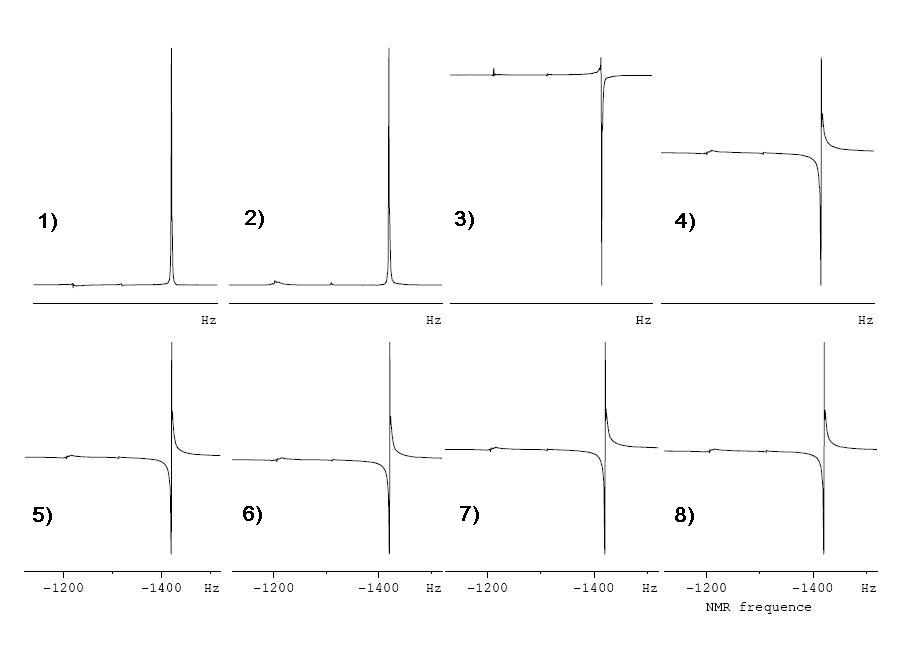
\includegraphics[width=0.99\columnwidth]{newspectrum}
\end{center}
\caption{Spectrums of the experiment. Starting from thermal
equilibrium, we first created a pseudopure state and the spectrum
after a read-out pulse on observed nuclear $^{1}H$ is showed as
Spectrum $1)$. We use the phase of this spectrum as a reference of
the successor spectrums. Spectrum $2)$ is obtained after adiabatic
evolution and the quantum state at this time is
$\frac{1}{\sqrt{2}}(|0\rangle+|1\rangle)\otimes|\psi\rangle$. As
showed in the figure, the spectrum is similar to that of PPS, which
is because that $|\psi\rangle$ is closed to state $|0\rangle$. The
following six spectrums are observed after the six iterations, which
present us visible phase information. The relative phase of each of
the six spectrums to Spectrum $2)$ are the experiment result of the
correspond iteration, that is, the phase is used to calculate the
parameter for the next iteration and to calculate the energy E.}
\label{newspectrum}
\end{figure}



%=================================experiment end========================================================

After each iterate the above procedure, we measure the phase shift
and thereby prepare the operator for the next iteration with the
scheme described before. Additionally, we stored the value
$\phi^{'}_k$ in each iteration for further use. After measured the
all six phases, we uses a recursive method to rebuild the $\phi$ as
the experiment result. The recursive method is formulate as follows,
$$
\phi^{result}_i=\phi^{result}_{i+1} / \phi_{errbd} + \phi^{'}_i,
\phi^{result}_5 = \phi_5,
$$
where $\phi_i$ is the measured phase in each iteration $i$ and the
method iterates from $i=5$ to $0$.

The result of the iteration is shown in Fig.\ref{expresult}a. The
value $\phi$ we got from experiment approaches the theoretical value
of $\phi$ with the iterations processing. But there're still a gap
between theoretical expectation and experimental value which could
be seen in the zoom-in part in Fig.\ref{expresult}a. The detail
information is listed in Tab.\ref{comparision} which shows the
precision of the binary value $\phi_{exp}$ in the iterations. Note
that, although we could get 18 bit value of $\phi$ in the overall
six iterations, only 17 bit is precise with theoretical
expectations. So the finally $\phi$ in our experiment is -1.851569,
a little different from theoretical value -1.8516.

The reason for this difference is the error caused by experimental
imperfections. As mentioned before, the evaluation could not be
arbitrarily precise because of the error in operation $U_k$. To this
end, we analyze the imperfection of $U_k$ and figured out the error
caused by this imperfection in Fig.\ref{expresult}b. So after the
5th iteration, the value will not be corrected as the $U_k$ caused
error is too large. Finally we get 17 bits of precise $\phi$ which
have already been the upper bound in our experiment.

\begin{figure}[htb]
\begin{center}
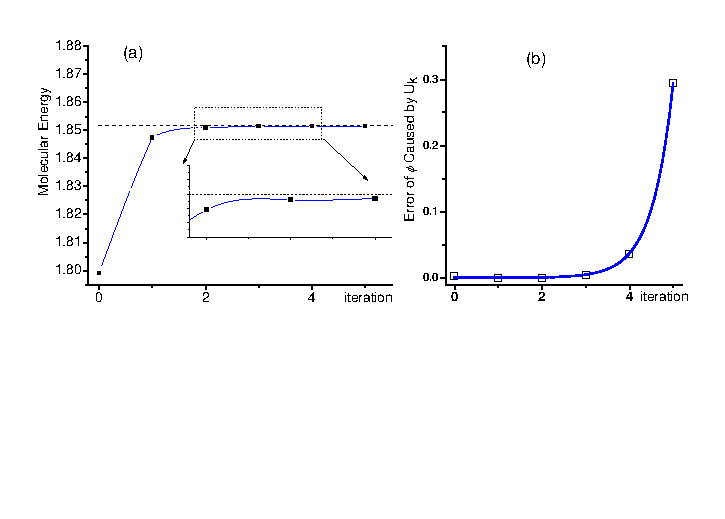
\includegraphics[width= 0.99\columnwidth]{expresult}
\end{center}
\caption{(a)The value $\phi$ approaches theoretical expectation as
the iteration performs. The green line is the fit of triangles which
denotes the experimental $\phi$ value in the iterations. The dash
red line is theoretical expectation of $\phi$. The experimental
value approaches theoretical expectation exponentially. (b) zooming
in part of the approaching process too show the limitation of
precision caused by experimental imperfection.(c) The error of
$\phi$ caused by imperfection of $U_k$ in our experiment. Because
the operation $U$ could not be arbitrarily precise, by applying $U$
with $8^k$ times, the error could be scale exponentially with
k.}\label{expresult}
\end{figure}

\begin{table}[htb]
\begin{center} {\footnotesize
\begin{tabular}{|c|c|ccccc|}
\hline
 & iteration & \multicolumn{5}{c}{binary values}\\
\hline
 \multirow{6}{*}{$\phi_{exp}$}
 & 0 & 0.01\underline{\textcolor{Red}{0}}00 & 11100 & 10010 & 11000 & 10010 \\
 &  1 & 0.01001 & \underline{\textcolor{Red}{0}}0100 & 00111 & 01110 & 01001\\
 &  2 & 0.01001 & 001\underline{\textcolor{Red}{0}}0 & 11001 & 01010 & 11010\\
 &  3 & 0.01001 & 00100 & 1\underline{\textcolor{Red}{1}}011 & 10011 & 10001\\
 &  4 & 0.01001 & 00100 & 1101\underline{\textcolor{Red}{1}} & 11110 & 11100\\
 &  5 & 0.01001 & 00100 & 11100 & 00\underline{\textcolor{Red}{0}}00 & 01001\\
\hline
\multicolumn{2}{|c|}{$\phi_{th}$} & 0.01001 & 00100 & 11100 & 00101 & 01100  \\
\hline
\end{tabular} }
\end{center}
\caption{\footnotesize The Comparison of $\phi$ in Theoretical
Expectation and Experimental result in the Iterations. All the
values are presented by binary value. The experiments get 3 more
bits in each iteration. The bits with an underline in each
$\phi_{exp}$ denotes the precision of the value. Overall, we get 17
bits of precision rather than 18 bits.} \label{comparision}
\end{table}

In conclusion, we simulate the $H_2$ molecule in our NMR quantum
computer. This is the first time simulating chemical interested
molecular energies in experiment. The result matches well with
theoretical expectation and we also find the precision limitation of
this algorithm in experiments which is caused by the imperfection of
operators. In fact, the extracted precision relies exponentially
with the precision of operator, which maybe the bottleneck of this
algorithm in applications.


This work was supported by National Nature Science Foundation of
China, The CAS, Ministry of Education of P.R.China, the National
Fundamental Research Program, and the DFG through Su 192/19-1.

\bibliography{quantum_simulation}

\end{document}
